\documentclass{beamer}

\mode<presentation>
{
  \usetheme{default}
  \usecolortheme{default}
  \usefonttheme{default}
  \setbeamertemplate{navigation symbols}{}
  \setbeamertemplate{caption}[numbered]
}

\usepackage[english]{babel}
\usepackage[utf8x]{inputenc}

\title[Short Title]{Beamer Template}
\author{Kentaro Wada}
\institute{Imperial College London}
\date{\today}

\begin{document}

\begin{frame}
  \titlepage
\end{frame}

\begin{frame}{Table of Contents}
  \tableofcontents
\end{frame}

\section{Introduction}
\begin{frame}{Introduction}
  Robotic Pick-and-Place
  \begin{itemize}
    \item Discriminate Picking
    \item Undiscriminate Picking
  \end{itemize}
\end{frame}

\section{Methods}
\begin{frame}{Proposed System}
  \begin{figure}
    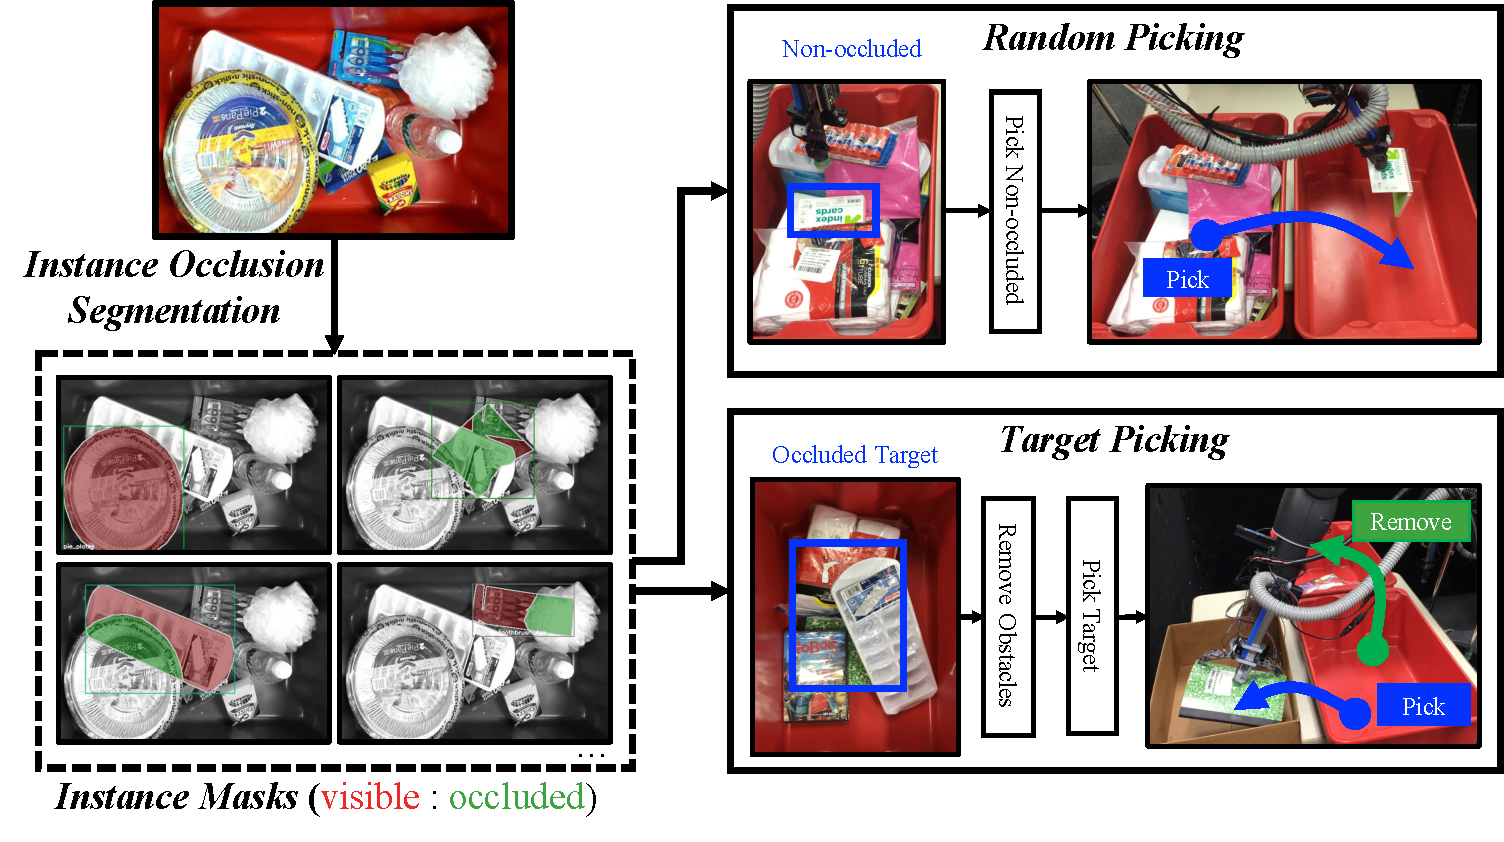
\includegraphics[width=\linewidth]{figs/overview.pdf}
    \caption{System Overview}
  \end{figure}
\end{frame}

\section{Experiments}
\begin{frame}{Experiments}
  This is what we conducted and got in the experiments.
\end{frame}

\section{Conclusions}
\begin{frame}{Conclusions}
  This is what we learned from experiments.
\end{frame}

\end{document}
